\documentclass[aspectratio=169]{beamer}

\mode<presentation>
{
  \usetheme{Madrid}
  \usecolortheme{default}
  \usefonttheme{default}
  \setbeamertemplate{navigation symbols}{}
  \setbeamertemplate{caption}[numbered]
}

\usepackage[english]{babel}
\usepackage[utf8]{inputenc}
\usepackage{booktabs}
\usepackage{amsmath}
\usepackage{tikz}

\title{Solving Takuzu via QAOA on a Native HUBO Formulation}
\subtitle{Quantum Optimization for Combinatorial Constraint Satisfaction}
\author{Ege Yurtsever}
\institute{Sabanc\i{} University}
\date{2026}

\begin{document}

\begin{frame}
  \titlepage
\end{frame}

\begin{frame}{Outline}
  \tableofcontents
\end{frame}

% ============================================================
\section{Introduction and Motivation}
% ============================================================

\begin{frame}{Motivation}

\begin{columns}
\begin{column}{0.55\textwidth}
\begin{itemize}
    \item Combinatorial optimization is ubiquitous in real-world applications
    \item Many such problems are \textbf{NP-hard}
    \item Quantum algorithms (QAOA) offer a promising heuristic framework
    \item \textbf{Challenge:} Encoding constraints into quantum-compatible forms
\end{itemize}

\bigskip
\textbf{Our goal:} Evaluate QAOA on a structured, NP-complete puzzle using a native higher-order formulation.
\end{column}

\begin{column}{0.4\textwidth}
\centering
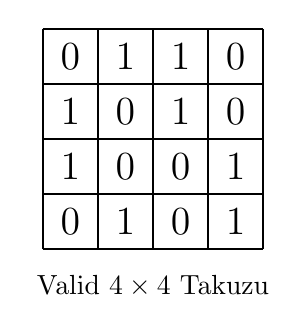
\begin{tikzpicture}[scale=0.7]
    \draw[thick] (0,0) grid (4,4);
    \node at (0.5,3.5) {\Large 0}; \node at (1.5,3.5) {\Large 1};
    \node at (2.5,3.5) {\Large 1}; \node at (3.5,3.5) {\Large 0};
    \node at (0.5,2.5) {\Large 1}; \node at (1.5,2.5) {\Large 0};
    \node at (2.5,2.5) {\Large 1}; \node at (3.5,2.5) {\Large 0};
    \node at (0.5,1.5) {\Large 1}; \node at (1.5,1.5) {\Large 0};
    \node at (2.5,1.5) {\Large 0}; \node at (3.5,1.5) {\Large 1};
    \node at (0.5,0.5) {\Large 0}; \node at (1.5,0.5) {\Large 1};
    \node at (2.5,0.5) {\Large 0}; \node at (3.5,0.5) {\Large 1};
    \node[below] at (2, -0.3) {Valid $4\times4$ Takuzu};
\end{tikzpicture}
\end{column}
\end{columns}
\end{frame}

% ============================================================
\section{Background}
% ============================================================

\begin{frame}{The Takuzu Puzzle}

\begin{columns}
\begin{column}{0.58\textwidth}
An $N \times N$ binary grid ($N$ even) subject to three rules:

\bigskip
\begin{enumerate}
    \item \textbf{Consecutive Limit:} No more than two identical values in a row/column
    \item \textbf{Equal Cardinality:} Each row/column has exactly $N/2$ zeros and $N/2$ ones
    \item \textbf{Uniqueness:} All rows distinct, all columns distinct
\end{enumerate}

\bigskip
\begin{alertblock}{Complexity}
The Takuzu decision problem is \textbf{NP-complete} [Berthier 2016], reduced from Not-All-Equal 3-SAT.
\end{alertblock}

\bigskip
For $N=4$: search space $= 2^{16} = 65{,}536$ configurations, only \textbf{72} valid solutions.
\end{column}

\begin{column}{0.38\textwidth}
\centering
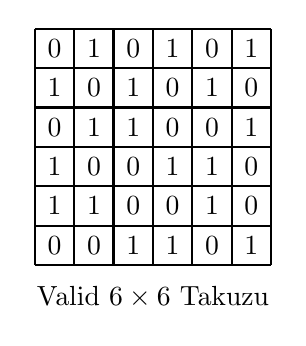
\begin{tikzpicture}[scale=0.5]
    \draw[thick] (0,0) grid (6,6);
    \node at (0.5,5.5) {0}; \node at (1.5,5.5) {1}; \node at (2.5,5.5) {0};
    \node at (3.5,5.5) {1}; \node at (4.5,5.5) {0}; \node at (5.5,5.5) {1};
    \node at (0.5,4.5) {1}; \node at (1.5,4.5) {0}; \node at (2.5,4.5) {1};
    \node at (3.5,4.5) {0}; \node at (4.5,4.5) {1}; \node at (5.5,4.5) {0};
    \node at (0.5,3.5) {0}; \node at (1.5,3.5) {1}; \node at (2.5,3.5) {1};
    \node at (3.5,3.5) {0}; \node at (4.5,3.5) {0}; \node at (5.5,3.5) {1};
    \node at (0.5,2.5) {1}; \node at (1.5,2.5) {0}; \node at (2.5,2.5) {0};
    \node at (3.5,2.5) {1}; \node at (4.5,2.5) {1}; \node at (5.5,2.5) {0};
    \node at (0.5,1.5) {1}; \node at (1.5,1.5) {1}; \node at (2.5,1.5) {0};
    \node at (3.5,1.5) {0}; \node at (4.5,1.5) {1}; \node at (5.5,1.5) {0};
    \node at (0.5,0.5) {0}; \node at (1.5,0.5) {0}; \node at (2.5,0.5) {1};
    \node at (3.5,0.5) {1}; \node at (4.5,0.5) {0}; \node at (5.5,0.5) {1};
    \node[below] at (3, -0.3) {Valid $6\times6$ Takuzu};
\end{tikzpicture}
\end{column}
\end{columns}
\end{frame}

\begin{frame}{HUBO and QUBO}

Both are ways to write an objective function over binary variables $x_i \in \{0,1\}$:

\bigskip
\begin{columns}
\begin{column}{0.48\textwidth}
\begin{block}{HUBO (Higher-Order)}
$$f(\mathbf{x}) = \sum_{S \subseteq \{1,\ldots,n\}} c_S \prod_{i \in S} x_i$$
\end{block}
\end{column}

\begin{column}{0.48\textwidth}
\begin{block}{QUBO (Quadratic)}
$$f(\mathbf{x}) = \sum_i a_i x_i + \sum_{i<j} b_{ij} x_i x_j$$
\end{block}
\end{column}
\end{columns}

\bigskip
QAOA can implement multi-qubit $Z$-interactions directly, so it can optimize a HUBO without reducing to QUBO. This saves us from introducing auxiliary variables.
\end{frame}

\begin{frame}{QAOA Overview}

\begin{center}
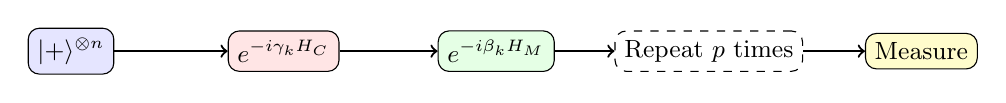
\begin{tikzpicture}[scale=0.9, every node/.style={font=\small}]
    \node[draw, rounded corners, fill=blue!10] (init) at (0, 0) {$|+\rangle^{\otimes n}$};
    \node[draw, rounded corners, fill=red!10] (uc) at (3, 0) {$e^{-i\gamma_k H_C}$};
    \node[draw, rounded corners, fill=green!10] (um) at (6, 0) {$e^{-i\beta_k H_M}$};
    \node[draw, dashed, rounded corners] (rep) at (9, 0) {Repeat $p$ times};
    \node[draw, rounded corners, fill=yellow!20] (meas) at (12, 0) {Measure};
    
    \draw[->, thick] (init) -- (uc);
    \draw[->, thick] (uc) -- (um);
    \draw[->, thick] (um) -- (rep);
    \draw[->, thick] (rep) -- (meas);
\end{tikzpicture}
\end{center}

\bigskip
\begin{itemize}
    \item $H_C$: Cost Hamiltonian (encodes the optimization objective)
    \item $H_M = \sum_i X_i$: Transverse-field mixer
    \item Parameters $(\gamma_1,\ldots,\gamma_p, \beta_1,\ldots,\beta_p)$ optimized classically
    \item Depth $p$ controls circuit expressibility
\end{itemize}
\end{frame}

% ============================================================
\section{Problem Formulation}
% ============================================================

\begin{frame}{HUBO Encoding of Takuzu}

Variables: $x_{r,c} \in \{0,1\}$ for each cell. Total: $N^2 = 16$ for $N=4$.

\bigskip
\textbf{1. No three consecutive identical values} (penalize ``111'' or ``000''):
$$H_{C1} = \underbrace{x_i x_{i+1} x_{i+2}}_{\text{= 1 iff all three are 1}} + \underbrace{(1{-}x_i)(1{-}x_{i+1})(1{-}x_{i+2})}_{\text{= 1 iff all three are 0}}$$

\bigskip
\textbf{2. Each row/column must have exactly $N/2$ ones} (zero iff count is correct):
$$H_{C2} = \underbrace{\left(\sum_{c=1}^N x_{r,c} - \frac{N}{2}\right)^2}_{\text{= 0 only when \#ones = N/2, else > 0}}$$

\bigskip
\textbf{3. All rows must be distinct} (penalize row $r$ = row $s$):
$$H_{C3} = \underbrace{\prod_{c=1}^N \bigl(2x_{r,c}x_{s,c} - x_{r,c} - x_{s,c} + 1\bigr)}_{\text{each factor = 1 iff } x_{r,c} = x_{s,c}\text{; product = 1 iff ALL columns match}}$$
\end{frame}

\begin{frame}{Complete HUBO Objective}

\begin{equation*}
    H_{\text{HUBO}} = P_1 \cdot H_{C1} + P_2 \cdot H_{C2} + P_3 \cdot H_{C3}
\end{equation*}

\bigskip
\begin{itemize}
    \item $P_1, P_2, P_3 > 0$ are penalty weights
    \item Valid Takuzu solution $\Leftrightarrow$ global minimum with energy $= 0$
    \item Only $N^2 = 16$ variables needed (no auxiliary variables!)
\end{itemize}

\bigskip
\begin{block}{Mapping to Qubits}
Substitution $x_i \rightarrow (I - Z_i)/2$ converts each HUBO monomial into weighted Pauli-$Z$ strings.

\medskip
Result: \textbf{145 Pauli terms} from 2505 HUBO monomials.
\end{block}
\end{frame}

\begin{frame}{Why Not QUBO?}

Rosenberg's method [1975] reduces degree by introducing auxiliary variables:

\bigskip
\begin{table}
\centering
\begin{tabular}{@{} lccc @{}}
    \toprule
    Grid & Primary Vars & Aux Vars (QUBO) & Total \\
    \midrule
    $4\times4$ & 16 & 196 & 212 \\
    $6\times6$ & 36 & 738 & 774 \\
    $8\times8$ & 64 & 1,832 & 1,896 \\
    \bottomrule
\end{tabular}
\end{table}

\bigskip
\begin{alertblock}{13$\times$ variable inflation for $N=4$}
Native HUBO: 16 qubits. QUBO: 212 qubits. Simulating 212 qubits is far beyond current classical or quantum hardware.
\end{alertblock}
\end{frame}

% ============================================================
\section{Implementation}
% ============================================================

\begin{frame}{Experimental Setup}

\begin{columns}
\begin{column}{0.48\textwidth}
\begin{block}{QAOA (Quantum)}
\begin{itemize}
    \item Qiskit Aer statevector simulator
    \item 16 qubits ($4\times4$ grid)
    \item Depths $p \in \{1, 2, 3\}$
    \item COBYLA optimizer (300 iter)
    \item 8192 measurement shots
    \item 3 trials per depth
\end{itemize}
\end{block}
\end{column}

\begin{column}{0.48\textwidth}
\begin{block}{RC2 SAT (Classical Baseline)}
\begin{itemize}
    \item PySAT library [Ignatiev 2019]
    \item CNF encoding (364 clauses)
    \item 128 variables (16 + 112 aux)
    \item Core-guided exact solver
    \item Guarantees optimality
    \item No HUBO/QUBO needed
\end{itemize}
\end{block}
\end{column}
\end{columns}

\bigskip
\textbf{Grid size limited to $N=4$}: statevector requires $2^{16}$ amplitudes. Full benchmark took $\sim$7 minutes.\\
For $N=6$ (36 qubits): statevector would need $2^{36} \approx 69$ billion amplitudes, estimated runtime $\sim$months on a single machine.
\end{frame}

% ============================================================
\section{Results and Analysis}
% ============================================================

\begin{frame}{QAOA Results: 9/9 Trials Found Valid Solutions}

\begin{table}
\centering
\begin{tabular}{@{} ccccc @{}}
    \toprule
    Depth $p$ & Best $\langle H \rangle$ & Mean $\langle H \rangle$ & Valid Solutions & Mean Time \\
    \midrule
    1 & 46.22 & 48.75 & 3/3 (100\%) & 21.97\,s \\
    2 & 46.64 & 50.53 & 3/3 (100\%) & 40.33\,s \\
    3 & 52.59 & 53.23 & 3/3 (100\%) & 43.87\,s \\
    \bottomrule
\end{tabular}
\end{table}

\bigskip
\begin{itemize}
    \item \textbf{100\% success rate} at all depths
    \item Best sampled bitstring always yields a valid Takuzu grid
    \item Each trial found a \emph{different} valid solution (sampling diversity)
    \item Expectation value $\neq 0$ (distribution spread), but ground states are sampled
\end{itemize}
\end{frame}

\begin{frame}{QAOA vs. Classical Solver}

\begin{table}
\centering
\begin{tabular}{@{} lccc @{}}
    \toprule
    Method & Variables/Qubits & Time & Valid \\
    \midrule
    QAOA ($p=1$) & 16 qubits & 21.97\,s & Yes \\
    QAOA ($p=2$) & 16 qubits & 40.33\,s & Yes \\
    QAOA ($p=3$) & 16 qubits & 43.87\,s & Yes \\
    RC2 SAT & 128 vars & 0.711\,ms & Yes \\
    \bottomrule
\end{tabular}
\end{table}

\bigskip
\begin{itemize}
    \item Classical solver: $\sim$30,000$\times$ faster (for $N=4$)
    \item \textbf{But:} QAOA timing = classical simulation overhead, not quantum hardware time
    \item SAT solvers exploit logical structure directly (no optimization landscape)
\end{itemize}
\end{frame}

\begin{frame}{Key Findings}

\begin{enumerate}
    \item \textbf{Native HUBO works.} QAOA successfully solves Takuzu without quadratization.
    
    \bigskip
    \item \textbf{Deeper circuits $\neq$ better.} $p=1$ outperforms $p=3$ (optimizer struggles with more parameters).
    
    \bigskip
    \item \textbf{13$\times$ qubit savings.} HUBO: 16 qubits vs. QUBO: 212 variables.
    
    \bigskip
    \item \textbf{High degeneracy helps.} 72 ground states out of 65,536 ($\approx 0.11\%$) makes sampling feasible.
    
    \bigskip
    \item \textbf{Classical dominates at small scale.} RC2 solves in sub-ms; quantum advantage needs larger instances.
\end{enumerate}
\end{frame}

% ============================================================
\section{Conclusion}
% ============================================================

\begin{frame}{Conclusion and Future Work}

\textbf{Contributions:}
\begin{itemize}
    \item Complete HUBO formulation of NP-complete Takuzu ($N^2$ variables only)
    \item Demonstrated native HUBO QAOA on 16 qubits with 100\% success
    \item Quantified 13$\times$ overhead of QUBO quadratization
    \item Comparative analysis against RC2 SAT solver
\end{itemize}

\bigskip
\textbf{Future Work:}
\begin{itemize}
    \item Extend to partially filled grids (the NP-complete decision variant)
\end{itemize}

\bigskip
\begin{block}{Code}
\url{https://github.com/evesfect/takuzu-optimization}
\end{block}
\end{frame}

\begin{frame}{References}
\footnotesize
\begin{itemize}
    \item E. Farhi et al., ``A Quantum Approximate Optimization Algorithm,'' arXiv:1411.4028, 2014.
    \item M. Berthier, ``The complexity of Takuzu puzzles,'' \textit{Theoretical Computer Science}, vol. 654, 2016.
    \item I. G. Rosenberg, ``Reduction of bivalent maximization to the quadratic case,'' 1975.
    \item S. Hadfield et al., ``From QAOA to a Quantum Alternating Operator Ansatz,'' \textit{Algorithms}, 2019.
    \item A. Ignatiev et al., ``RC2: An efficient MaxSAT solver,'' \textit{JSAT}, 2019.
    \item A. Lucas, ``Ising formulations of many NP problems,'' \textit{Frontiers in Physics}, 2014.
\end{itemize}
\end{frame}

\begin{frame}{}
\centering
\vfill
{\Large \textbf{Thank You}}

\bigskip
{\large Questions?}

\bigskip
\texttt{ege.yurtsever@sabanciuniv.edu}
\vfill
\end{frame}

\end{document}
